\documentclass{article}
\usepackage{blindtext}
\usepackage[utf8]{inputenc}
\usepackage{graphicx}
\usepackage{hyperref}
\usepackage[dvipsnames]{xcolor}
\usepackage{fancyvrb}
\graphicspath{ {/home/abhinav/Desktop/} }
 \hypersetup{
    colorlinks=true,
    linkcolor=blue,
    pdfpagemode=FullScreen,
}
\title{\textbf{General Linear Congruence Generator}}
\author{Abhinav Gupta}
\date{\today}

\begin{document}
 \tableofcontents
\maketitle

\section{Short Summary}
 
General Linear Congruence Generator

\[x_{i+1}=(ax_i+b) mod m\]
\[u_{i+1}=x_{i+1}/m\]
\[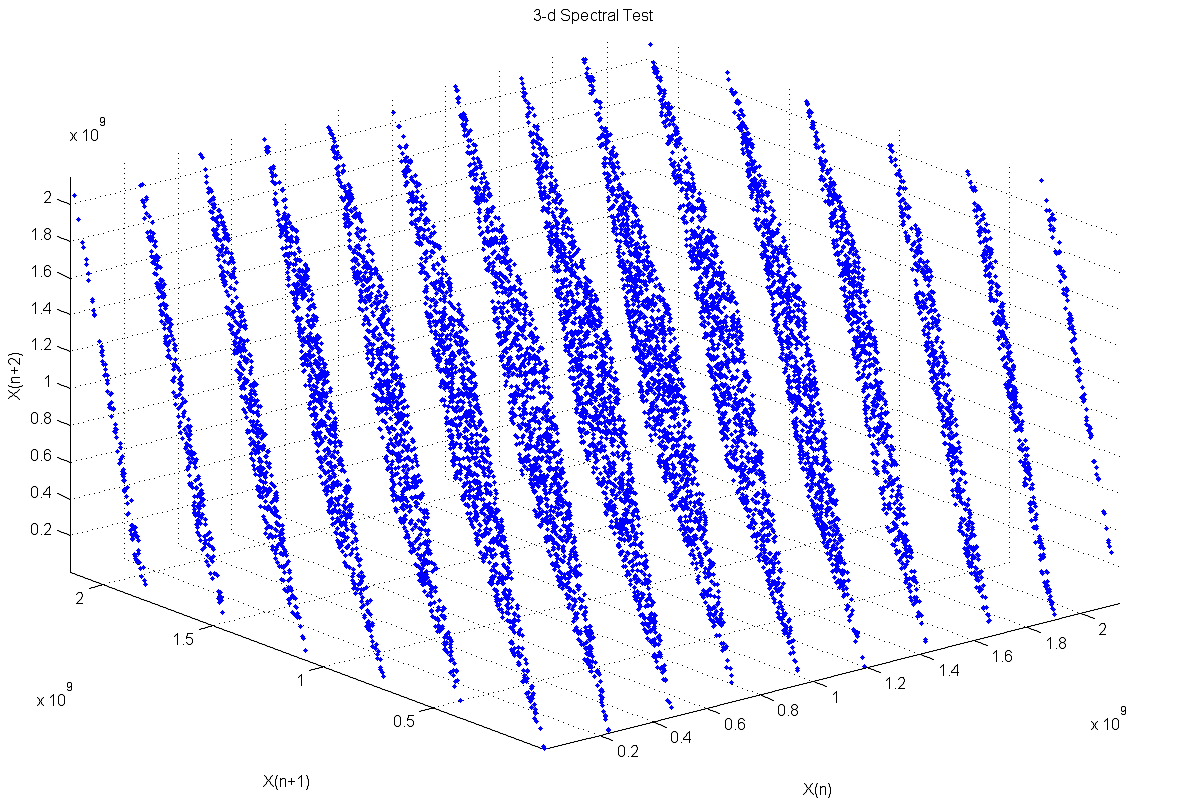
\includegraphics[scale=.4]{glcg}\]
\(x_i\) is a sequence of pseudo-random values\\
\(m\) is \textbf{modulus}\\
\(a\) is \textbf{multiplier}\\
\(b\) is \textbf{increment}\\
\(x_0\) is \textbf{"Seed" or start value}


A linear congruential generator (LCG) is an algorithm that yields a sequence of pseudo-randomized numbers calculated with a discontinuous piecewise linear equation. The method represents one of the oldest and best-known pseudo-random number generator algorithms. The theory behind them is relatively easy to understand, and they are easily implemented and fast, especially on computer hardware which can provide modulo arithmetic by storage-bit truncation.
\section{Question-1}
 
When a=3, b=0 and m=11 \(-->\) 5 different values are generated.\\
When a=6,b=0 and m=11 \(-->\) 10 different values are generated.\\
The reason is as regardless of what \textbf{'seed'} we choose same values start getting generated when \(x_{i+1}=seed\) . So after repetitive modulus of '6' and '3', the following sequences is formed :

\[6\ 3\ 7\ 9\ 10\ 5\ 8\ 4\ 2\ 1\ 6\ \]
\[3\ 9\ 5\ 4\ 1\ 3\ \]

So to generate a sequence of random numbers it would be better to use  a=6,b=0 and m=11 data-set as they generate more number of different numbers.
\begin{itemize}
\item Problems:\\
1-- Cycle is mostly shorter due to small m.\\
2-- Generating not much randomness in numbers.\\


\item \textbf{"C++  Code is as follows: "}
\end{itemize}
\VerbatimInput{ass2-question1.cpp}
\vspace{5mm}

\section{Question-2}
\textbf{"Generated bar-graph for frequencies of values falling within different-different ranges : "}
\begin{itemize}
\item Observations:
In Linear Congruence Generator is look-alike uniform as probability of finding a random number generated in a range is almost equal for all ranges (i.e. random values generated are uniformly generated over the range modulus "m")
\item a=1597 and seed=1000 (all different values):
\[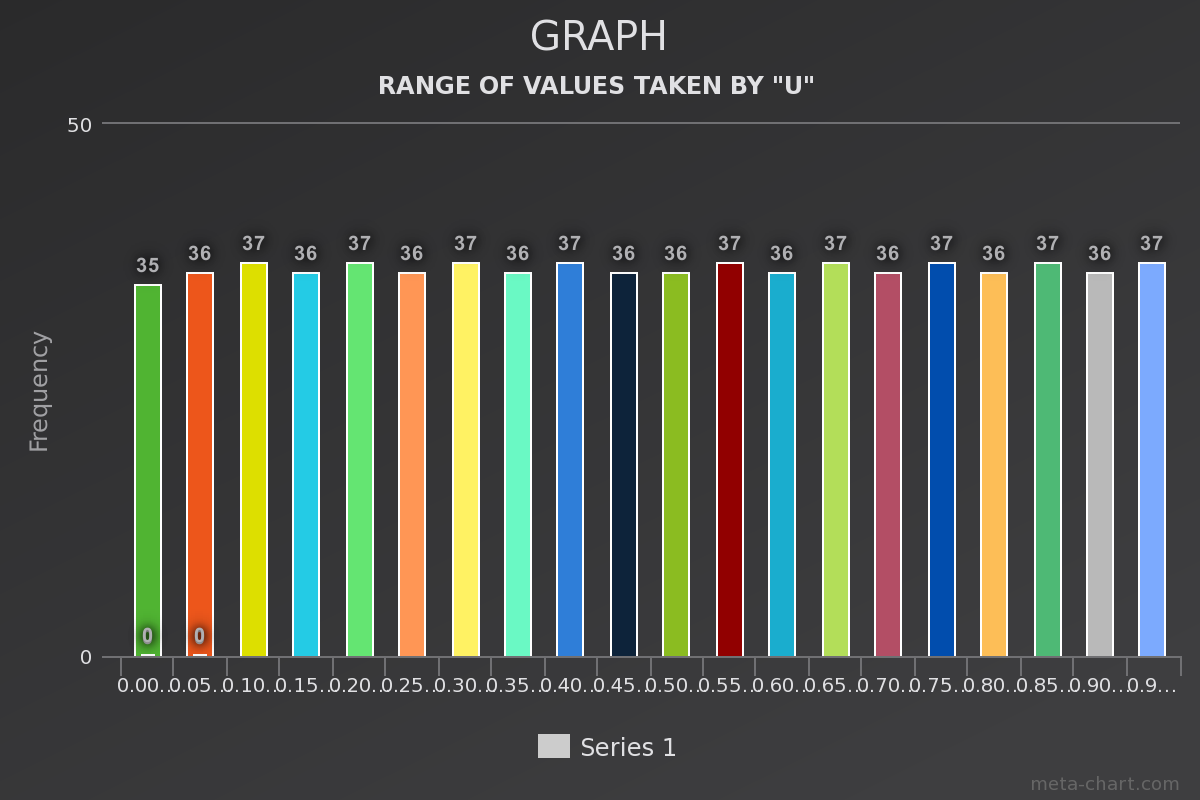
\includegraphics[scale=.3]{1597-1000}\]
\item a=1597 and seed=10005 (all different values):
\[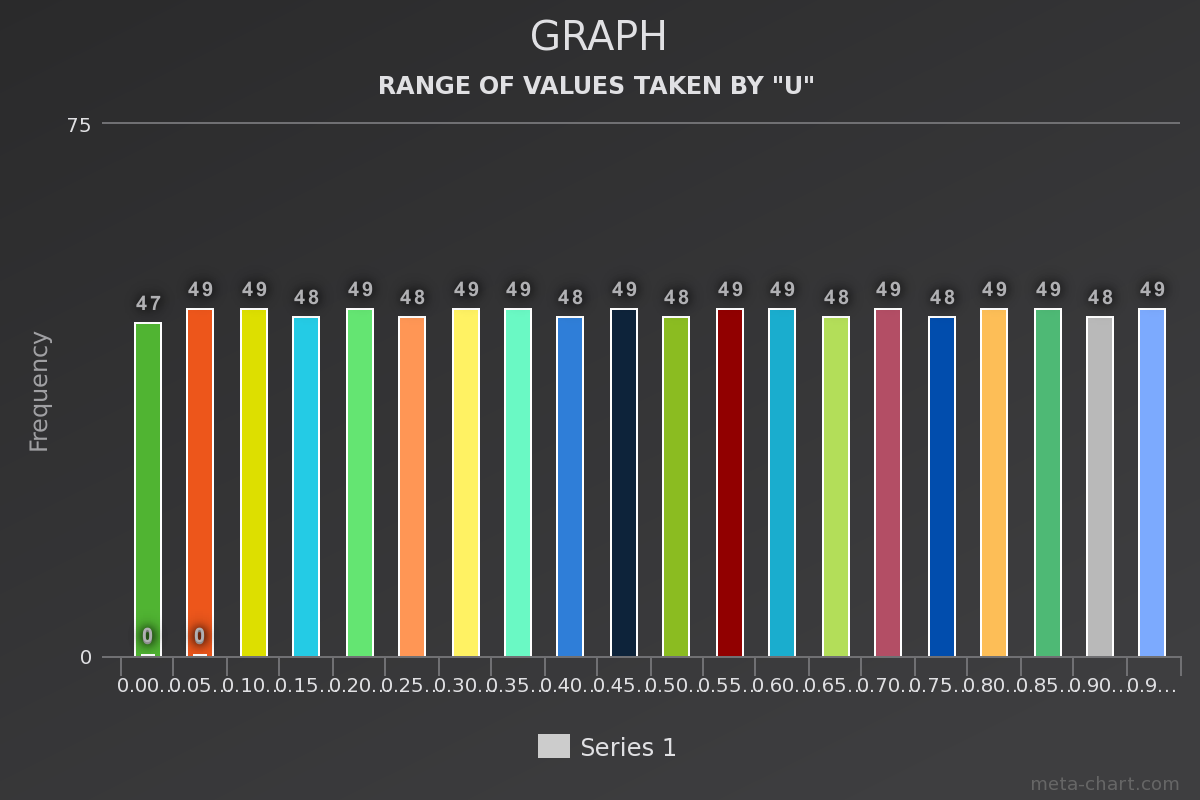
\includegraphics[scale=.3]{1597-10005}\]
\item a=1597 , output- 100000 values (same as well as different), seed=77177:
\[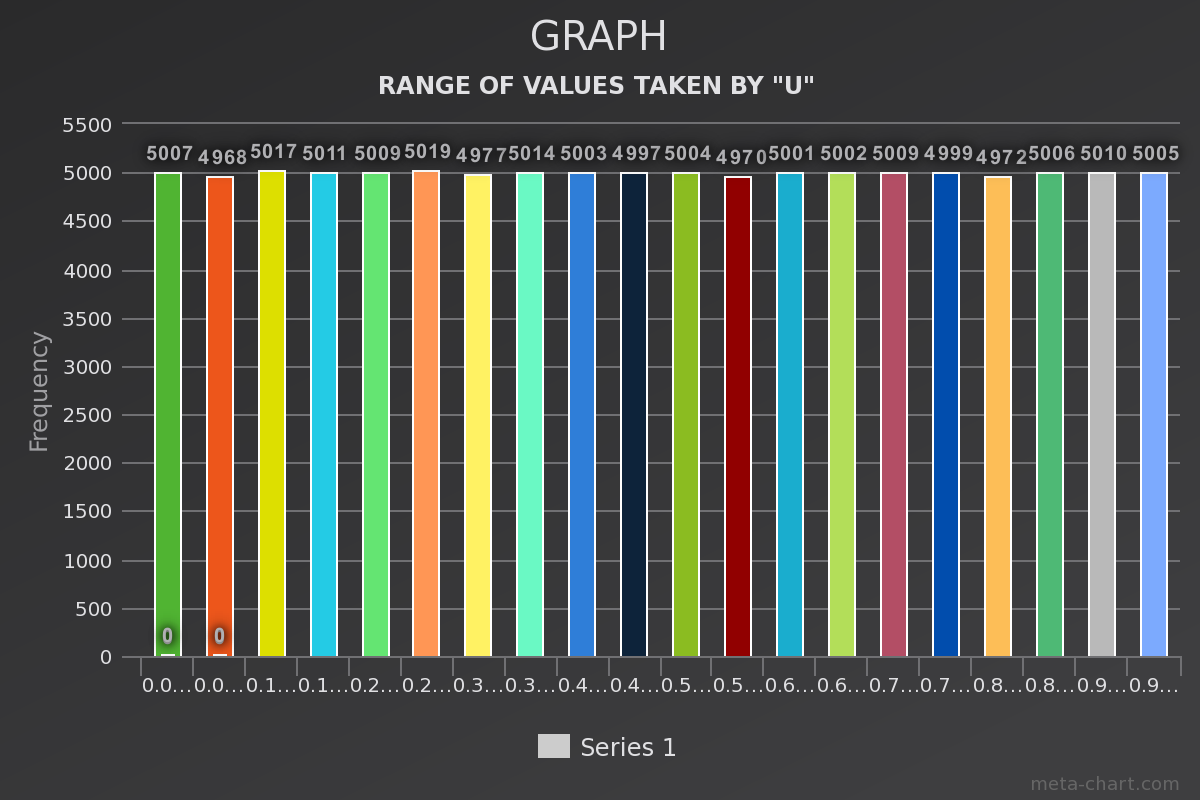
\includegraphics[scale=.3]{1597-100000-77177}\]
\item a=51749 and seed=2:
\[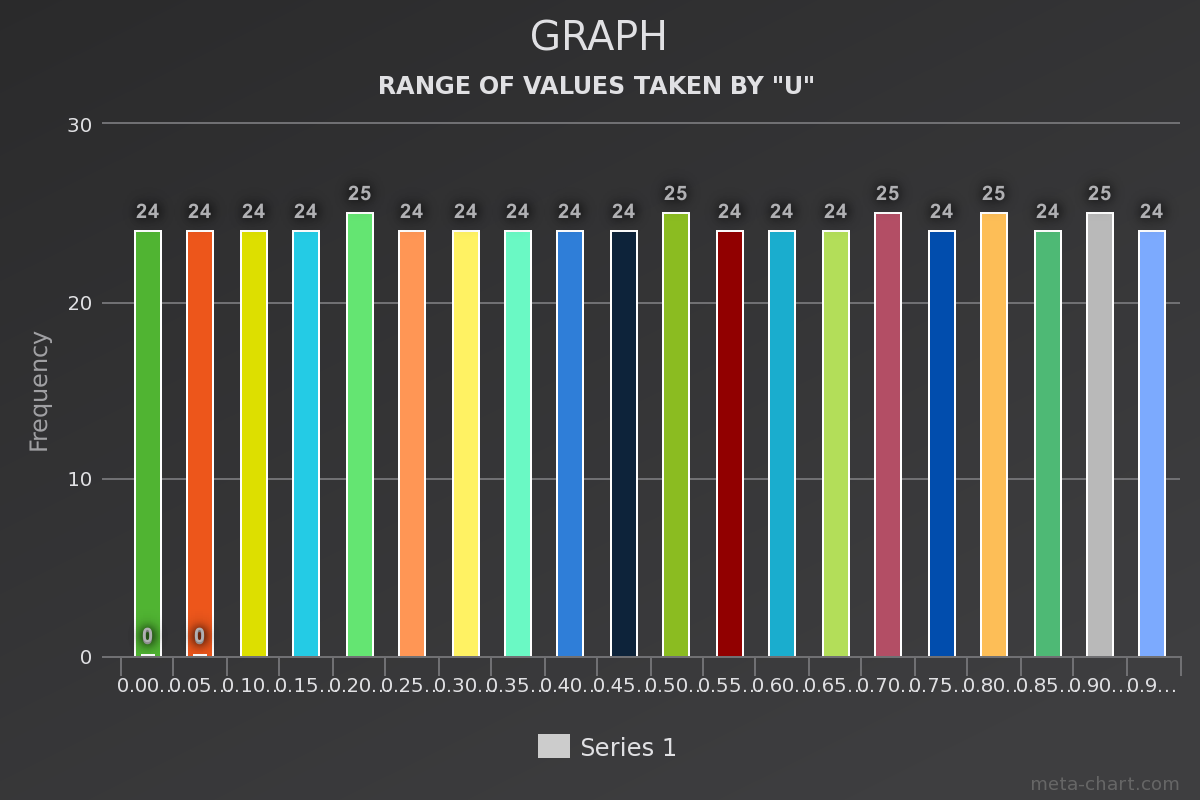
\includegraphics[scale=.3]{51749-2}\]
\item a=51749 and seed=359:
\[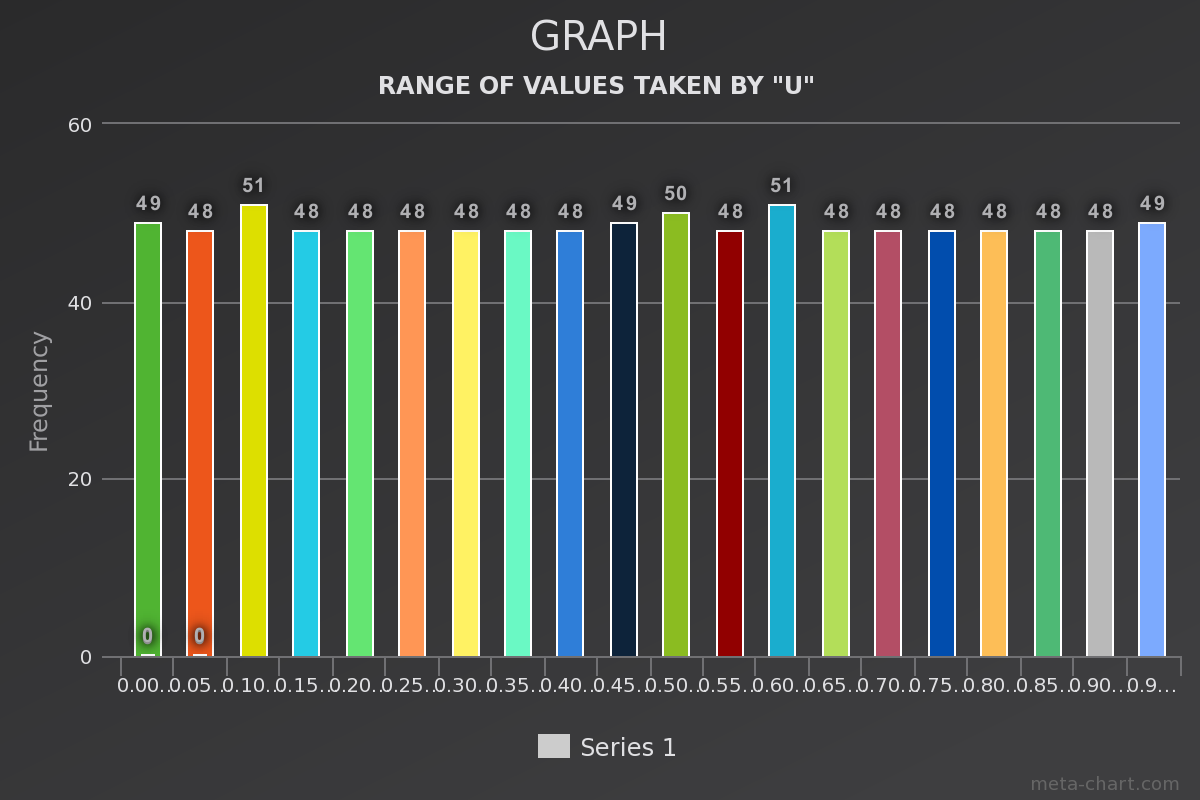
\includegraphics[scale=.3]{51749-359}\]
\item \textbf{"C++ code is as follows : "}
\VerbatimInput{ass2-question2.cpp}
\end{itemize}
\vspace{20mm}
\section{Question-3}
\begin{itemize}
\item Observation:\\
For the Linear Congruence Generator to be truly a \textbf{"Uniform Distribution"}, the distribution of graph points would have been uniformly scattered over the unit square (or cube) but that is not the case here as points are lying over some specific hyperplanes and are not scattered. 
\item Scattered Plot:
\[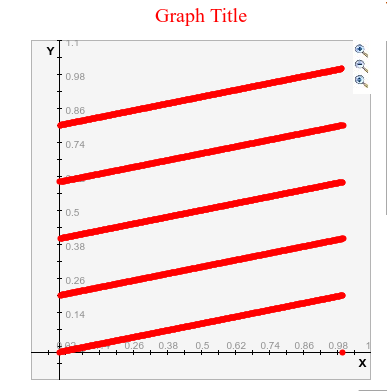
\includegraphics[scale=.5]{graph}\]
\item GnuPlot
\[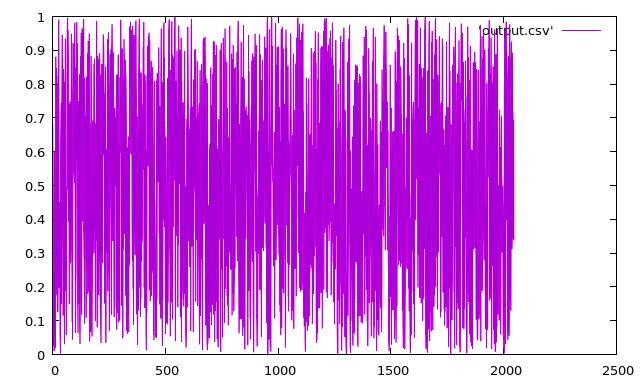
\includegraphics[scale=.5]{gnuplot}\]
\\
\item \textbf{"C++ code is as follows : "}
\VerbatimInput{ass2-question3.cpp}
\end{itemize}
 
\end{document}